\documentclass{article}
\usepackage{url}
\usepackage{fancyhdr}
\usepackage{amsmath, amsfonts, amsthm, amssymb}  
\usepackage{secdot}
\usepackage{epsfig}
\usepackage{lastpage}
\usepackage{hyperref}
\usepackage{graphicx}
\usepackage{color}
\usepackage{epstopdf}
\usepackage{fancyvrb}

\usepackage{geometry}
\geometry{letterpaper, left=1in, right=1in, top=1in, bottom=1in}

\pagestyle{fancy}
\fancyhf{}
\renewcommand{\headrulewidth}{0pt}
\rfoot{\thepage/\pageref{LastPage}}
\lhead{OSU ECEN 4233 - High-Speed Computer Arithmetic - Spring 2021}
\lfoot{\LaTeX}

\begin{document}

\title{Wallace Multiplier Example}
\author{James E. Stine \\
Electrical and Computer Engineering Department\\
Oklahoma State University \\
Stillwater, OK 74078, USA}
\date{}

\maketitle
%\thispagestyle{plain}\pagestyle{plain}

\section{Wallace Multiplier}
This document is meant to show the in-class example of a $6$-bit by $6$-bit
Wallace Multiplier.  Figure~$2$ shows usually how industry
documents it.  The reorganization of the partial product matrix into an
inverted triangle is also usually eliminated for industrial documents, but I
kept it in mainly because I did not want to waste time deleting it.  Here is
a table documenting the area where the final iteration has an $8$-bit CPA:
  \begin{table} [h]
    \centering
    \begin{tabular}{|c|c|c|c|c|c|c|c|c|c|} \hline
    Iteration & Number of $(3,2)$ Counters & Number of $(2,2)$ Counters & Row Height
      \\ \hline \hline
      1 & 8 & 4 & 6 \\ \hline
      2 & 5 & 4 & 4 \\ \hline
      3 & 3 & 5 & 3 \\ \hline \hline
  Total & 16 & 13 & - \\ \hline
    \end{tabular}
  \end{table}

Please note that the major difference between Figure~$2$ and
Figure~$1$ is that Figure~$2$ does not contain
the ovals that I utilized in class.  The ovals are something I use to help me
figure out where the $(3,2)$ and $(2,2)$ counters go.  You are welcome to use
your own method to help you in creating Wallace multipliers.  The methodology
for creating Wallace trees, or so they are called, can
be organized into the following steps listed below.  Usually, Wallace trees or
diagrams do not contain the final CPA, because it is implied.
\begin{enumerate}
\item Reorganize matrix into inverted triangle (optional)
\item Group the rows into sets of $3$.
\item Starting at far right column, use $(2,2)$ and $(3,2)$ counters as long 
each subset of $3$, has at least $3$ rows.
\item Repeat step $(3)$ until the final height is $2$.
\end{enumerate}

  \begin{figure}
    \begin{center}
      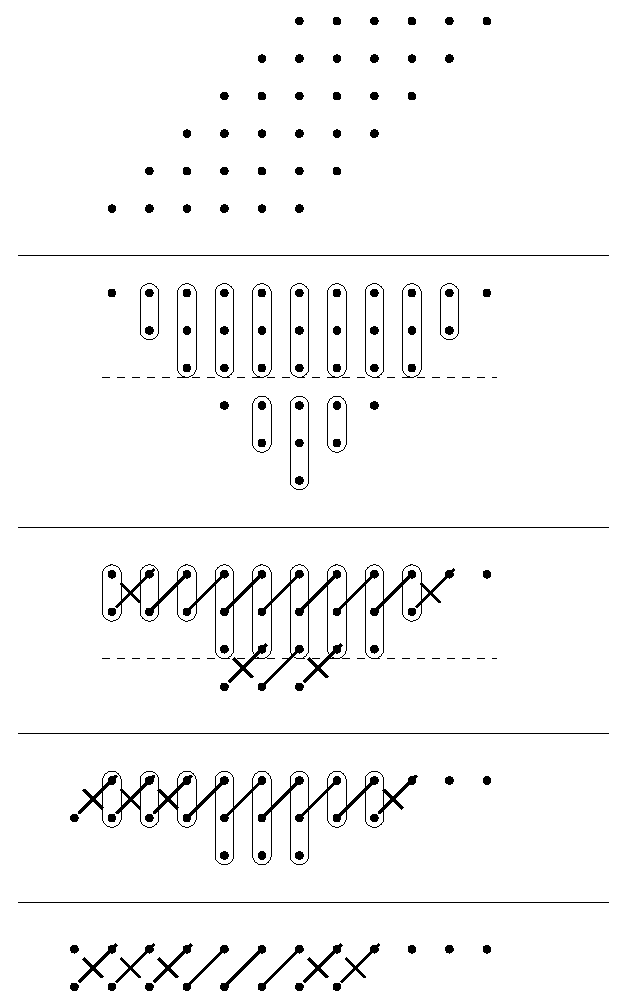
\includegraphics[scale=1.0]{wallace6.eps}
    \end{center}
    \label{wallace6.fig}
    \caption{In-class Example of $6 \times 6$ Wallace Multiplier.}
  \end{figure}

  \begin{figure}
    \begin{center}
      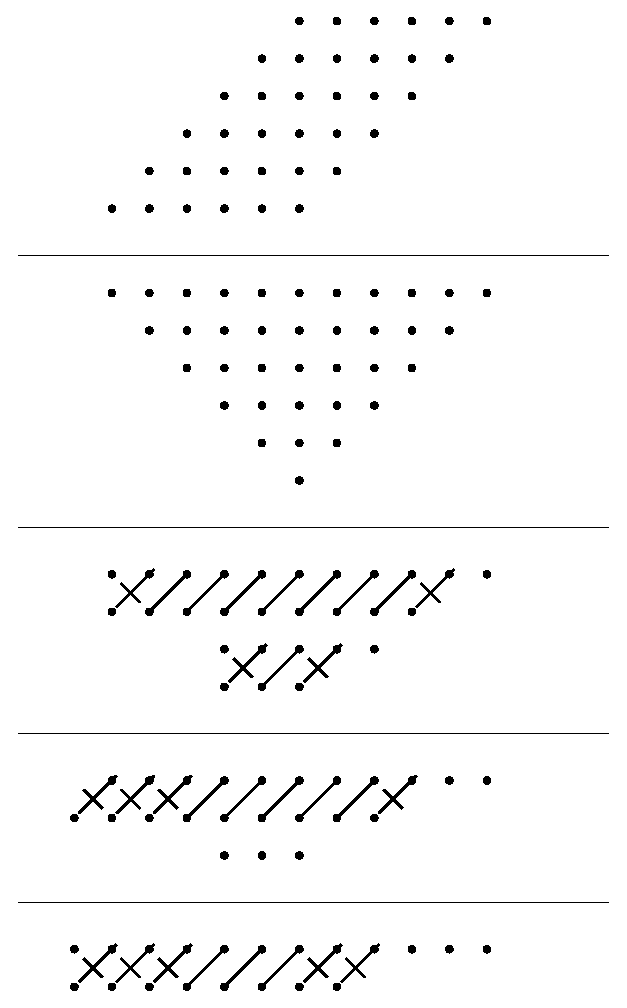
\includegraphics[scale=1.0]{wallace6l.eps}
    \end{center}
    \label{wallace6l.fig}
    \caption{In-class Example of $6 \times 6$ Wallace Multiplier (how usually
    described in literature).}
  \end{figure}

\end{document}
